\documentclass{beamer}
\title{Git Basics}
\author{David Kouka}
\date{\today}

\usepackage{graphicx}   % For including images
\usepackage{listings}   % For code listings
\usepackage{tikz}       % For diagrams
\usetikzlibrary{positioning}

\lstset{
    basicstyle=\ttfamily\color{blue}, % Change color and font
    keywordstyle=\color{red},
    commentstyle=\color{green},
    stringstyle=\color{orange},
    columns=flexible,
    keepspaces=true,
    showstringspaces=false,
}

\begin{document}

\frame{\titlepage}  % Title slide

\section{Table of Contents}

\begin{frame}
\tableofcontents
    \begin{center}
        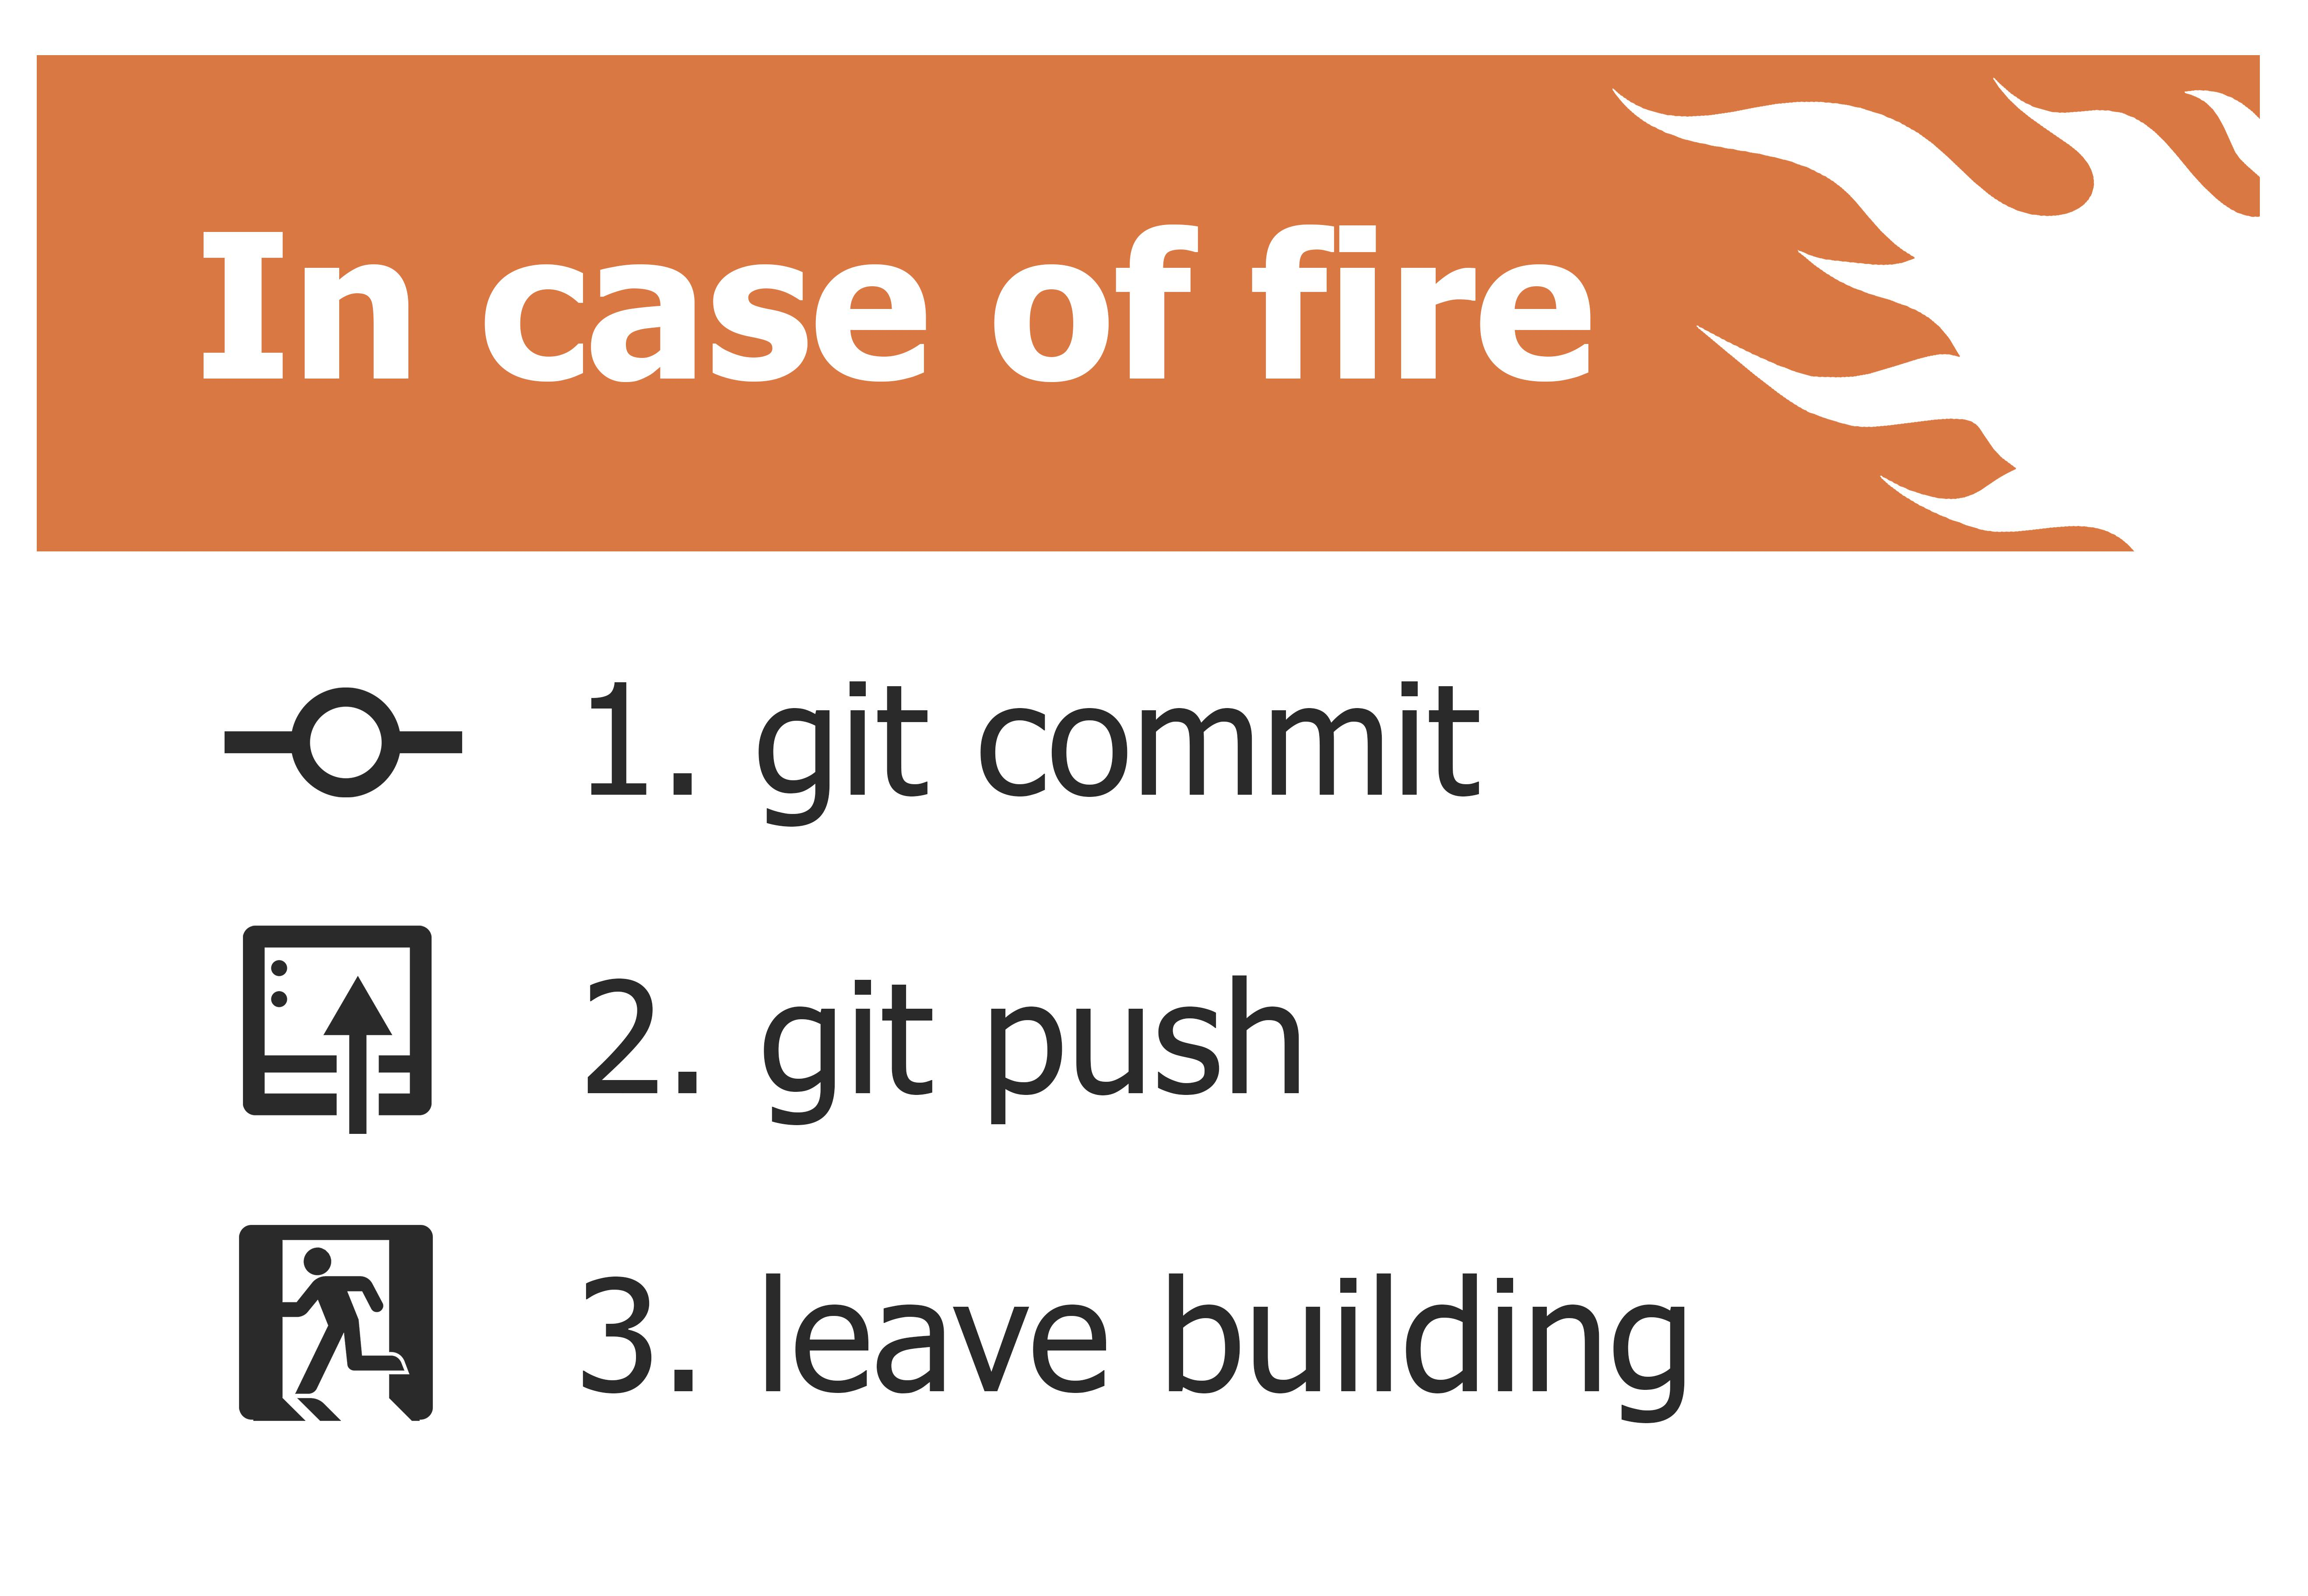
\includegraphics[width=0.5\linewidth]{img/in_case_of_fire.jpg}
    \end{center}
%TODO
\end{frame}

\section{Version control}

\begin{frame}{Why using version control}
    \begin{itemize}
        \item<1-> Tracking changes \lstinline{git diff}
        \item<2-> Backup and recovery \lstinline{git checkout}
        \item<3-> Collaborative work (authors, conflicts, PR)
        \item<4-> Accountability \lstinline{git blame}
        \item<5-> "Documentation" via commit messages \lstinline{git log}
        \item<6-> Safe experiments \lstinline{git branch}
        \item<7-> Easy release management (tags, banches, CI/CD, ...)
    \end{itemize}
\end{frame}

\section{Git commands}

\subsection{Cloning}

\begin{frame}{git clone}
    \only<1-> Copy repository from server

    \begin{tikzpicture}[
            roundnode/.style={circle, draw=green!60, fill=green!5, very thick, minimum size=7mm},
            squarednode/.style={rectangle, draw=red!60, fill=red!5, very thick, minimum size=5mm},
        ]
        \only<2->{
            \node[draw, roundnode] (local) {local};
        }
        \only<3->{  % Only show the remote node on slide 3 and up
            \node[squarednode] (remote) [right=of local] {remote};
            \draw[->] (local.east) -- (remote.west);  % Draw the arrow to the remote node
        }
    \end{tikzpicture}


    \begin{itemize}
        \item<4-> Bitbucket 
        \item<5-> Gitea
        \item<6-> Github
        \item<7-> Gitlab
    \end{itemize}
\end{frame}

\end{document}

